\documentclass[a4paper, 12pt]{article}
\usepackage[utf8]{inputenc}
\usepackage{myshortcuts}
\usepackage{a4wide}
\usepackage{mhchem}
\usepackage{physics}
\usepackage{csquotes}
\usepackage{enumitem}
\usepackage{etoolbox}
\usepackage{multirow}
\usepackage[british]{babel}
\usepackage[labelfont=bf]{caption}
\usepackage[caption=false]{subfig}
\usepackage[style=numeric,backend=biber]{biblatex}
\usepackage[separate-uncertainty=true, multi-part-units=single]{siunitx}

\allowdisplaybreaks

\sisetup{detect-all = true}
\addbibresource{mysources.bib}

\title{
\textbf{Physics Internal Assessment}\\
\bigskip
What is the diffraction pattern when \SI{650}{\nm} laser is obstructed by thin wires of varying widths?
}
\author{}
\date{}

\begin{document}
\maketitle

\section*{Introduction}
The phenomenon of optical diffraction can be roughly defined as the bending of light   (as waves) around an aperture or the corners of an obstacle.

\section*{Theory}

Babinet's principle \cite{babinet}: 
\begin{displayquote}
    ``Suppose that the eye observes a point source of light. If a small opaque object is placed just off the line of sight, the effects of this object is the same as that of a precisely similar aperture illuminated from the same source.''
\end{displayquote}

\newpage

\section*{Materials}
\begin{itemize}
\itemsep 0em
    \item Tape
    \item Millimetre paper (\SI{1.0+-.5}{\mm} squares)
    \item Measuring tape (precision: \SI{+-.05}{\cm})
    \item Monochromatic laser diode (wavelength: \SI{650+-10}{\nm} \cite{laser-specs})
    %TODO 38 < 40
    \item Diapositive for diffraction: 6 slits of width varying between \SI{40}{\um} and \SI{400}{\um}
    \item Wire-holding stand: 6 wires of of width varying between \SI{40}{\um} and \SI{150}{\um} \cite{wires-specs}
\end{itemize}

\begin{figure}[H]
    \centering
    \minipage{0.5\textwidth}
        \centering
        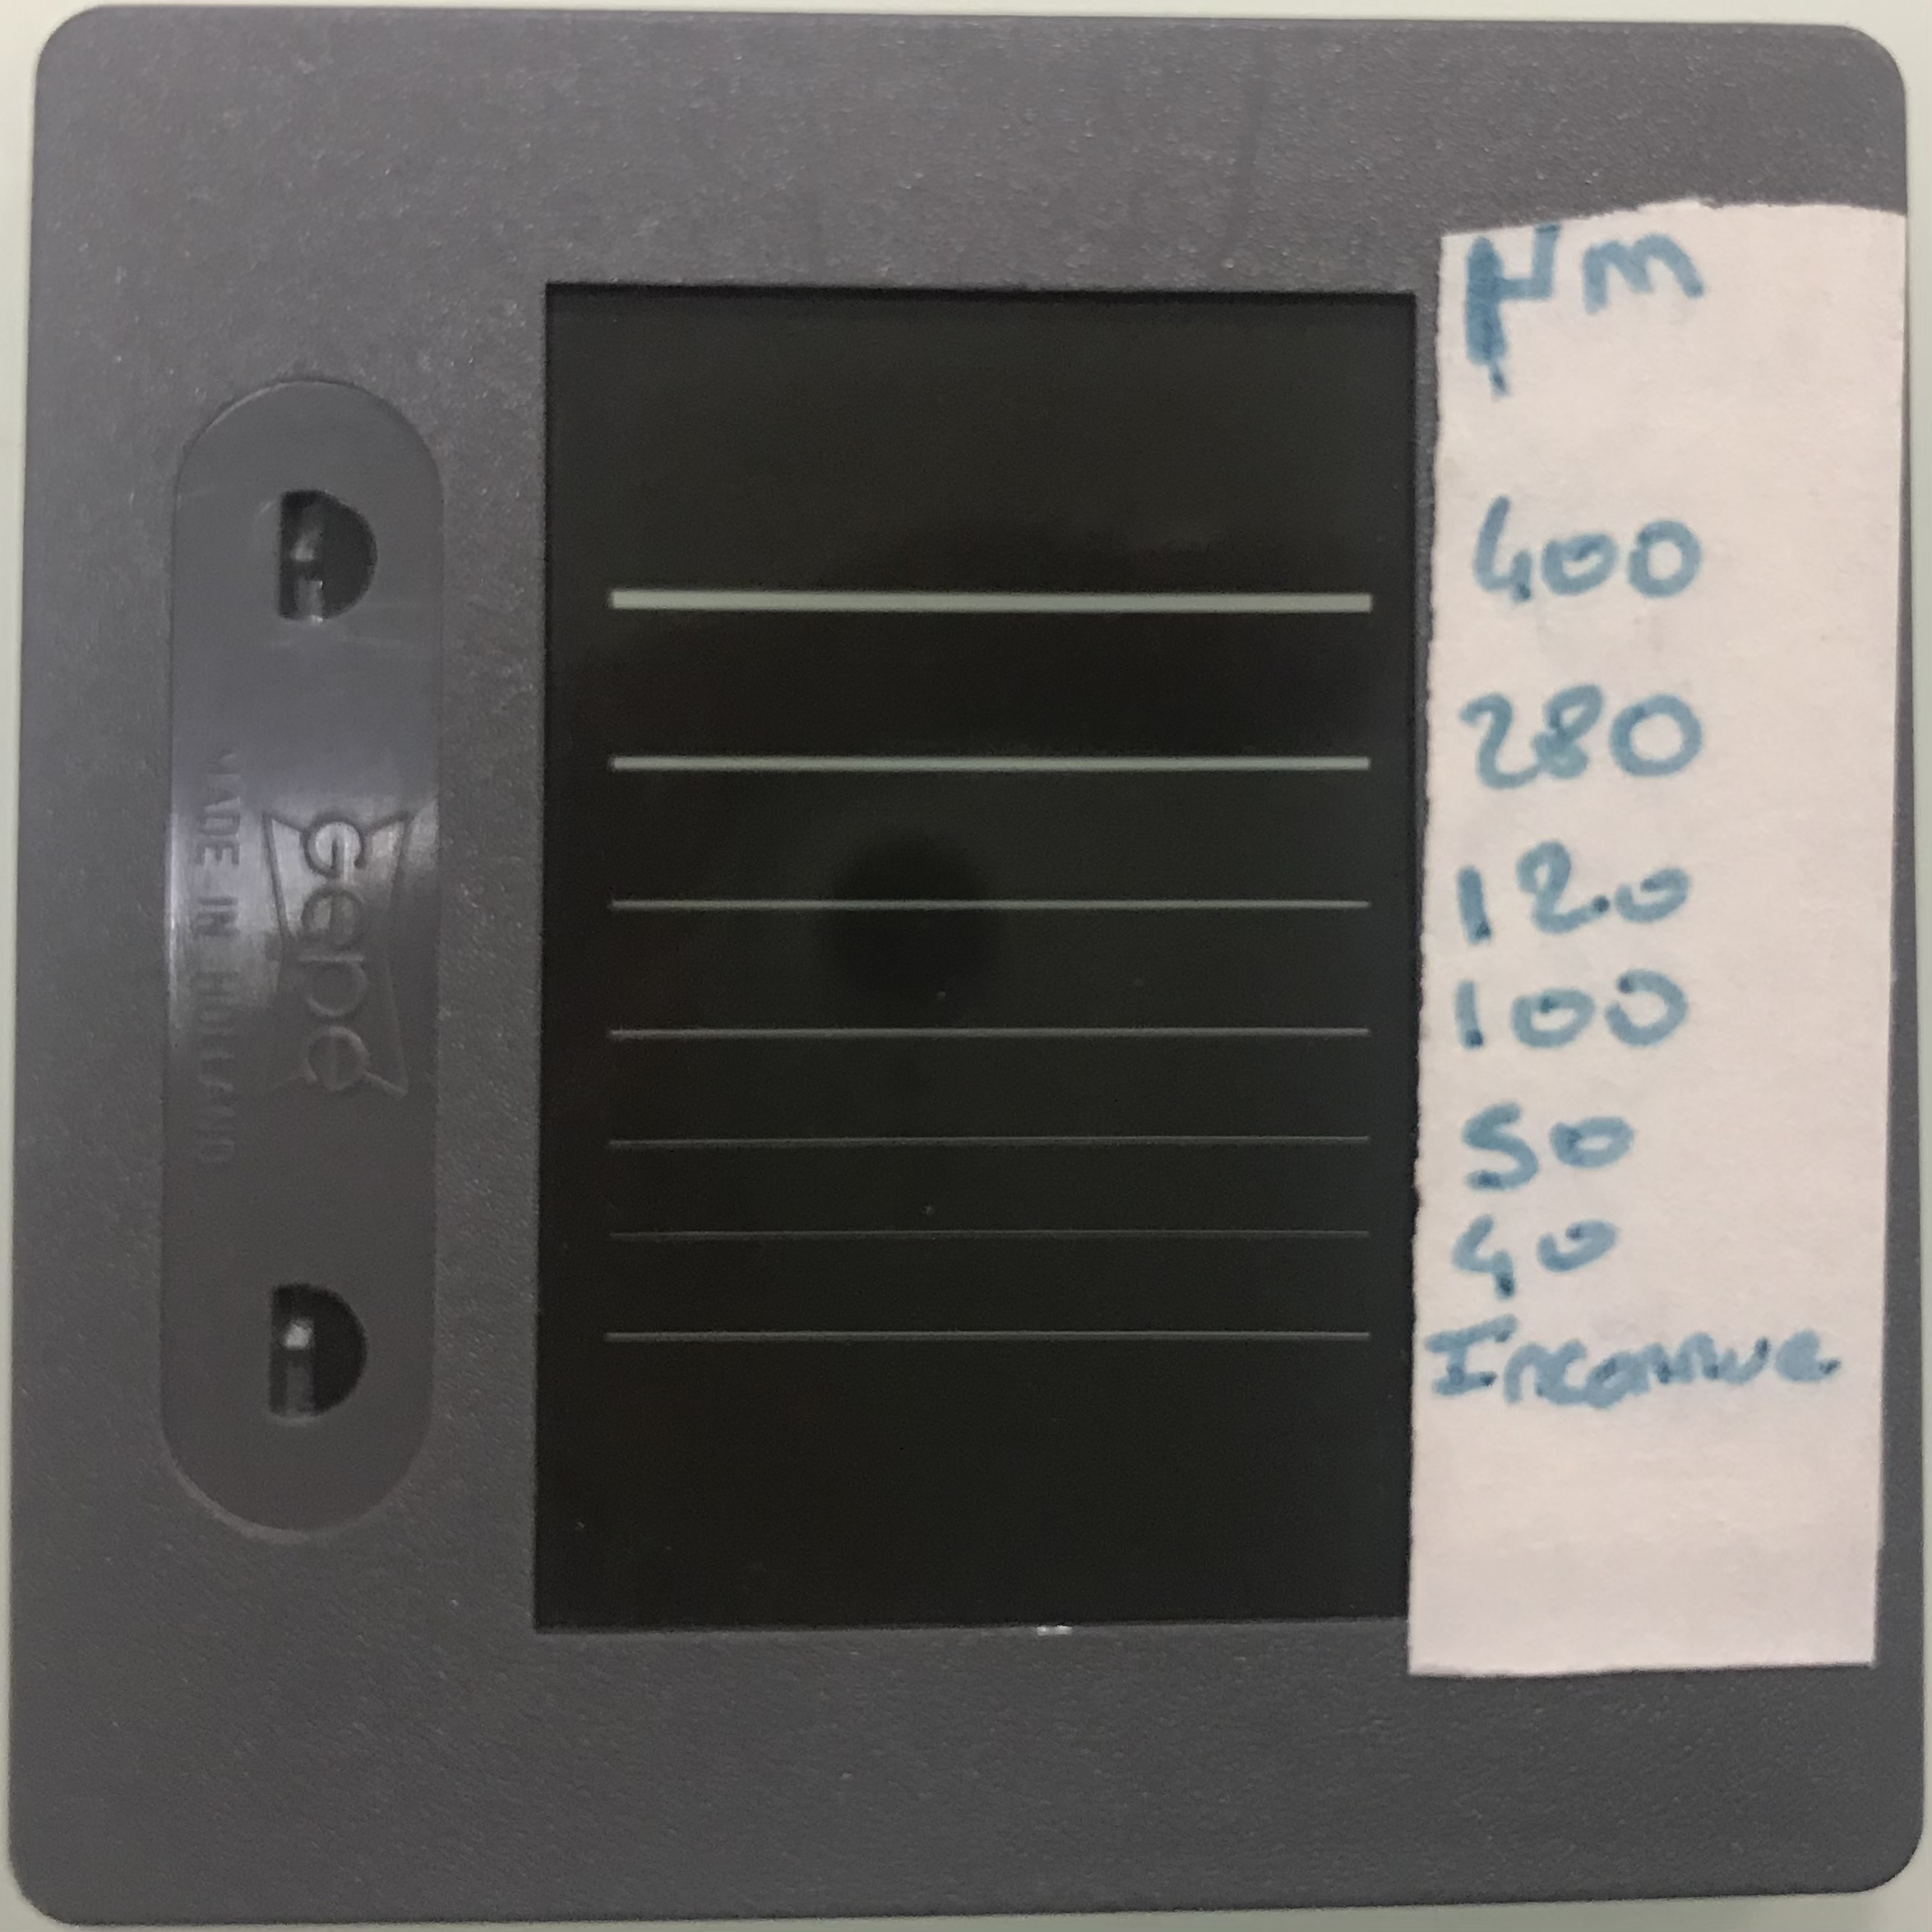
\includegraphics[width=.85\textwidth]{img/slits}
    \endminipage\hfill
    \minipage{0.5\textwidth}
        \centering
        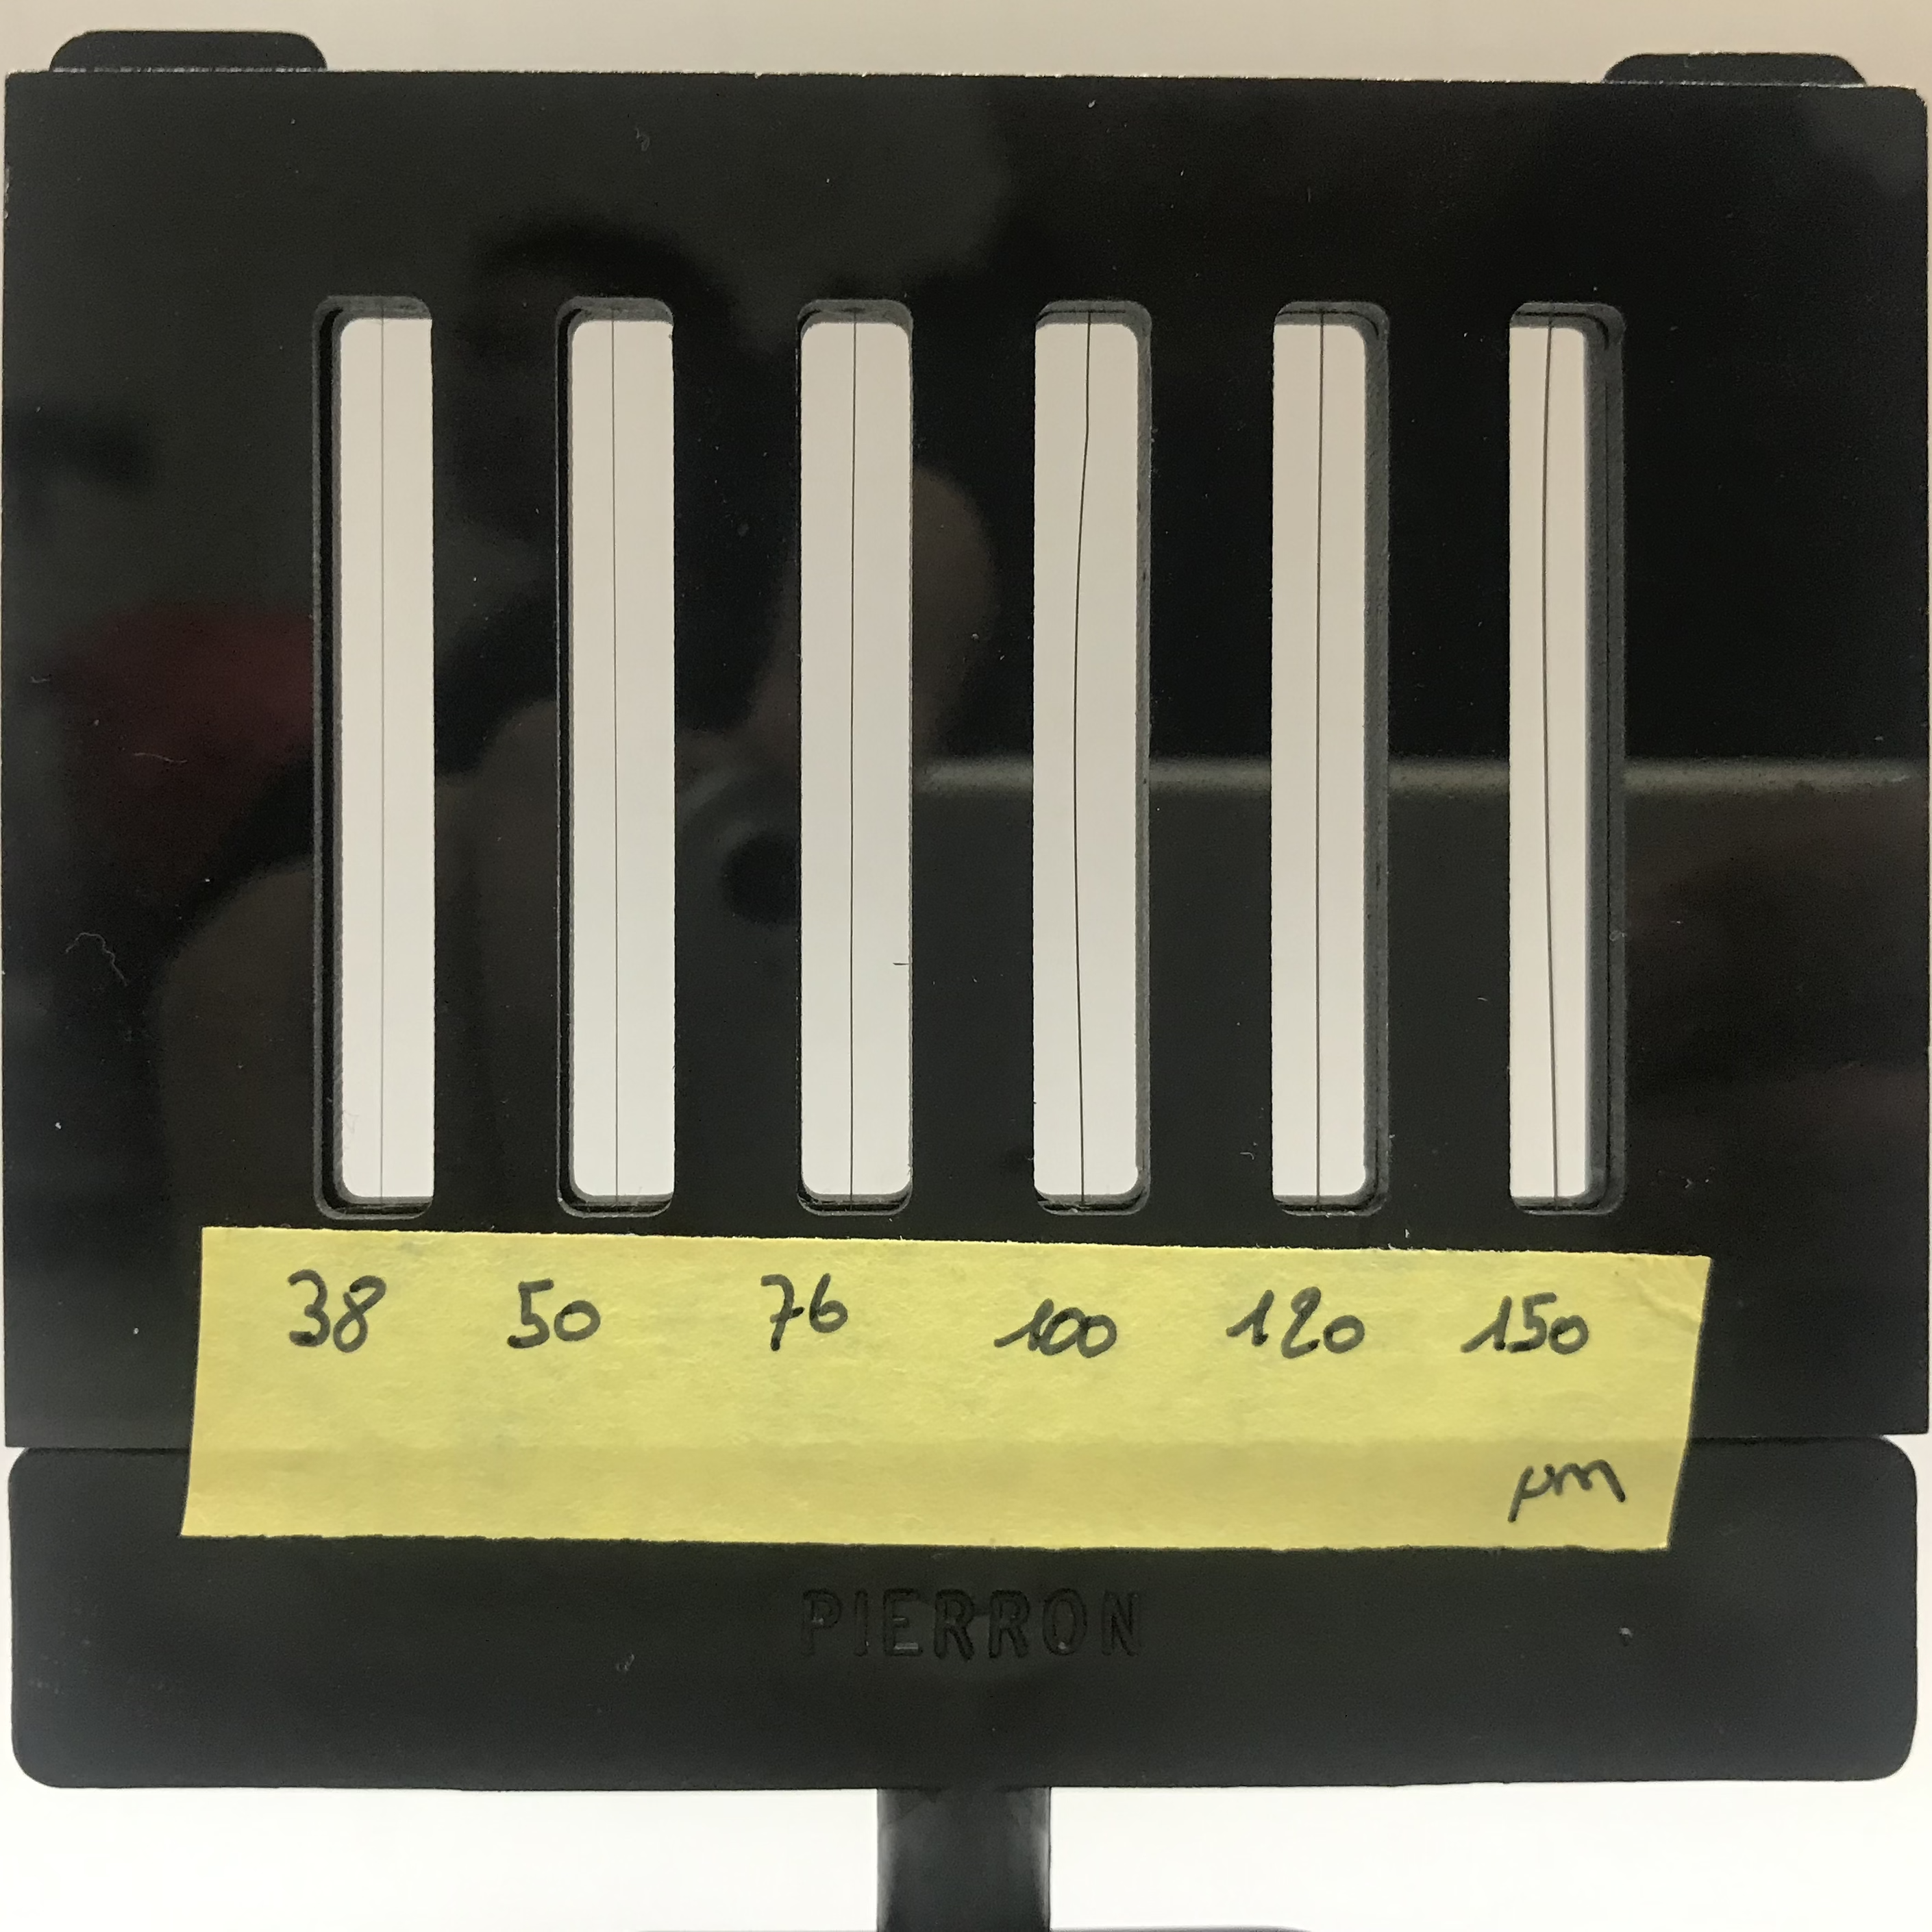
\includegraphics[width=.85\textwidth]{img/wires}
    \endminipage\hfill
    \caption{Test test. }
    \label{fig:slits-wires}
\end{figure}

\section*{Method}
To minimise the impact of ambient lighting on the diffraction pattern observed, the experiment is carried out in a dark room. Since the pupil then dilates to improve vision by allowing more light into the eye, special care should be taken to avoid shining the laser beam or its reflection into the eye. Possible measures to prevent eye damages include ensuring that no one else is in the same room and not pointing the laser on reflective surfaces.

\begin{enumerate}
\itemsep 0em
    \item Fix the end of the measuring tape between the table and the wall, and extend the tape in a straight line up to the other end of the table.
    \item Using the reading from the measuring tape, place the middle of the stand (where the wires are located) at a distance of \SI{2.50}{\m} away from the wall. \label{step:place-stand}
    \item Set up the laser diode behind the stand so that the wire obstructs the laser beam by padding the diode with one or two thick books from below if needed (see \cref{fig:setup}). Turn on the laser diode. \label{step:place-laser}
    \item Tape a piece of millimetre paper on the wall, aligning the centre of the paper with the laser beam while avoiding looking into the laser beam.
    \item Take at least 3 pictures of the millimetre paper on which the diffraction pattern is observed. \label{step:get-pattern}
    \item Move the stand so that another wire of a different width is obstructing the laser beam. Make sure that the distance between the wires and the wall remains to be \SI{2.50}{\m}. Repeat step \ref{step:get-pattern}. \label{step:change-wire}
    \item Repeat step \ref{step:change-wire} until the diffraction pattern of all 6 wires are recorded. \label{step:iterate-wire}
    \item Take the millimetre paper and the tapes off from the wall. Turn off the laser diode. \label{step:clean-up}
    \item Replace the wire-holding stand with the diapositive with slits mounted on another stand. Repeat steps \ref{step:place-stand}--\ref{step:iterate-wire}.
    \item Clean up following the instructions from \ref{step:clean-up}. Put away the experimental apparatus.
\end{enumerate}

\begin{figure}[H]
    \centering
    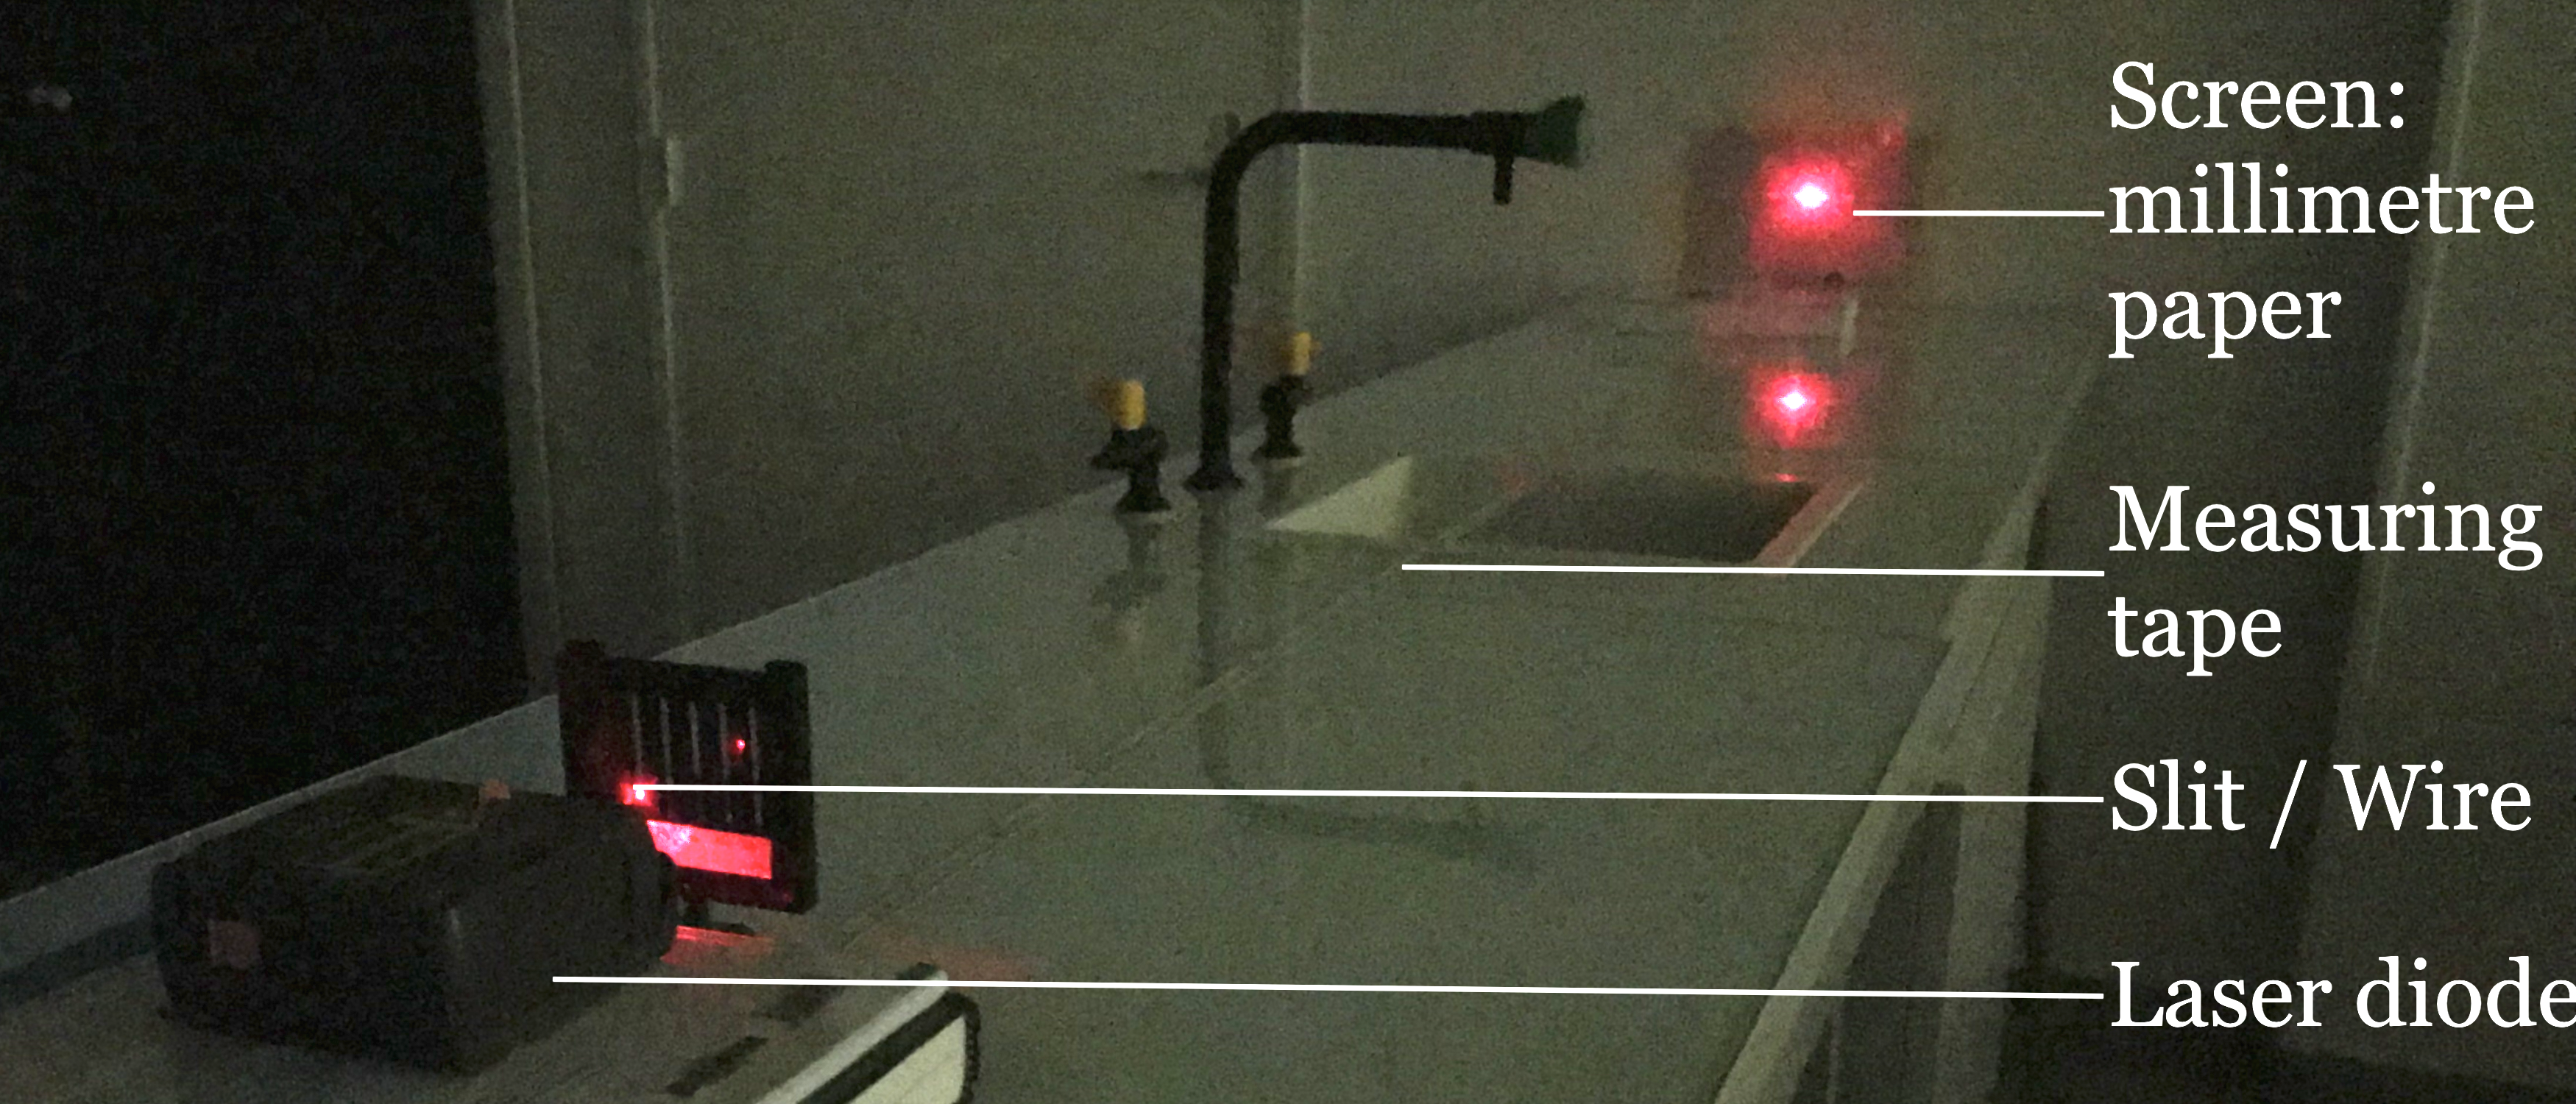
\includegraphics[width=\textwidth]{img/setup}
    \caption{Setup of the experiment. The exposure is modified for better visibility. }
    \label{fig:setup}
\end{figure}

\section*{Raw Data}
\begin{figure}[H]
    \renewcommand{\thesubfigure}{1a}
    \subfloat[Wire; $\text{width} = \SI{38}{\um}$.]{
        \includegraphics[width=0.48\textwidth]{img/wires/38}
    }
    \renewcommand{\thesubfigure}{1b}
    \subfloat[Slit; $\text{width} = \SI{40}{\um}$.]{
        \includegraphics[width=0.48\textwidth]{img/slits/40}
    }
    
    \renewcommand{\thesubfigure}{2a}
    \subfloat[Wire; $\text{width} = \SI{50}{\um}$]{
        \includegraphics[width=0.48\textwidth]{img/wires/50}
    }
    \renewcommand{\thesubfigure}{2a}    
    \subfloat[Slit; $\text{width} = \SI{50}{\um}$]{
        \includegraphics[width=0.48\textwidth]{img/slits/50}
    }

    \renewcommand{\thesubfigure}{3a}
    \subfloat[Wire; $\text{width} = \SI{100}{\um}$]{
        \includegraphics[width=0.48\textwidth]{img/wires/100}
    }
    \renewcommand{\thesubfigure}{3b}
    \subfloat[Slit; $\text{width} = \SI{100}{\um}$]{
        \includegraphics[width=0.48\textwidth]{img/slits/100}
    }

    \renewcommand{\thesubfigure}{4a}    
    \subfloat[Wire; $\text{width} = \SI{120}{\um}$]{
        \includegraphics[width=0.48\textwidth]{img/wires/120}
    }
    \renewcommand{\thesubfigure}{4b}
    \subfloat[Slit; $\text{width} = \SI{120}{\um}$]{
        \includegraphics[width=0.48\textwidth]{img/slits/120}
    }
    
    \caption{Diffraction patterns produced by slits and wires of similar or identical widths. }
    \label{fig:patterns}
\end{figure}

Qualitatively, the geometry of the diffraction pattern produced when the laser beam is obstructed by a single thin wire is indeed identical to that of the single-slit diffraction pattern: both consist of a series of dark and bright fringes, contain a central bright fringe corresponding to the principle maximum, and demonstrate that the intensity of subsequent maxima decreases significantly. A discrepancy occurs at the centre of the central bright fringe -- the wire diffraction pattern clearly shows the 2D Gaussian distribution of the laser beam's intensity, while the slit diffraction pattern does not. This can be explained by the fact that the width of the slit containing the wire (\SI{4.5}{\mm} \cite{wire_measurement}) is much bigger than the width of the diffraction slit (\SI{40}{\um}--\SI{400}{\um}) and allows more light to pass through.


\section*{Processed Data}
One advantage of having pictures of the diffraction patterns in a digital format is that the experimental data can be processed with computer programs using OpenCV \cite{opencv_library}.

Firstly, a Python script \cite{py_extract} is devised to find the main axis of the diffraction pattern:

\begin{figure}[H]
    \centering
    \includegraphics[width=\textwidth]{scripts/processed-data/axis}
    \caption{Main axis (blue line) of the diffraction pattern. Slit; $\text{width} = \SI{100}{\mm}$. }
    \label{fig:mains-axis}
\end{figure}

Since the laser beam is red, the BLUE and GREEN channels may be omitted, and the RED channel of the image is extracted. Then, for each pixel along the main axis, the intensity (between 0 and 255, both ends included) is recorded and stored in an array. The results obtained by transforming one picture for each trial are shown below. 

\begin{figure}[H]
    \renewcommand{\thesubfigure}{a}
    \subfloat[Wire; $\text{width} = \SI{38}{\um}$.]{
        \includegraphics[width=0.48\textwidth]{scripts/processed-data/wires/38}
    }
    \renewcommand{\thesubfigure}{g}
    \subfloat[Slit; $\text{width} = \SI{40}{\um}$.]{
        \includegraphics[width=0.48\textwidth]{scripts/processed-data/slits/40}
    }
    
    \renewcommand{\thesubfigure}{b}
    \subfloat[Wire; $\text{width} = \SI{50}{\um}$.]{
        \includegraphics[width=0.48\textwidth]{scripts/processed-data/wires/50}
    }
    \renewcommand{\thesubfigure}{h}
    \subfloat[Slit; $\text{width} = \SI{50}{\um}$.]{
        \includegraphics[width=0.48\textwidth]{scripts/processed-data/slits/50}
    }

    \renewcommand{\thesubfigure}{c}
    \subfloat[Wire; $\text{width} = \SI{76}{\um}$.]{
        \includegraphics[width=0.48\textwidth]{scripts/processed-data/wires/76}
    }
    \renewcommand{\thesubfigure}{i}
    \subfloat[Slit; $\text{width} = \SI{100}{\um}$.]{
        \includegraphics[width=0.48\textwidth]{scripts/processed-data/slits/100}
    }

    \renewcommand{\thesubfigure}{d}
    \subfloat[Wire; $\text{width} = \SI{100}{\um}$.]{
        \includegraphics[width=0.48\textwidth]{scripts/processed-data/wires/100}
    }
    \renewcommand{\thesubfigure}{j}
    \subfloat[Slit; $\text{width} = \SI{120}{\um}$.]{
        \includegraphics[width=0.48\textwidth]{scripts/processed-data/slits/120}
    }

    \renewcommand{\thesubfigure}{e}
    \subfloat[Wire; $\text{width} = \SI{120}{\um}$.]{
        \includegraphics[width=0.48\textwidth]{scripts/processed-data/wires/120}
    }
    \renewcommand{\thesubfigure}{k}
    \subfloat[Slit; $\text{width} = \SI{280}{\um}$.]{
        \includegraphics[width=0.48\textwidth]{scripts/processed-data/slits/280}
    }

    \renewcommand{\thesubfigure}{f}
    \subfloat[Wire; $\text{width} = \SI{150}{\um}$.]{
        \includegraphics[width=0.48\textwidth]{scripts/processed-data/wires/150}
    }
    \renewcommand{\thesubfigure}{l}
    \subfloat[Slit; $\text{width} = \SI{400}{\um}$.]{
        \includegraphics[width=0.48\textwidth]{scripts/processed-data/slits/400}
    }
    
    \centering
    \includegraphics[width=\textwidth]{scripts/processed-data/colour-bar.png}
    
    \caption{Variation in RED intensity along the main axis of the diffraction pattern. }
    \label{fig:processed-patterns}
\end{figure}

\begin{figure}[H]
    \centering
    \includegraphics[width=\textwidth]{img/data}
    \caption{Width of the central bright fringe versus the width of wire or slit. }
    \label{fig:data}
\end{figure}

\section*{Results}

\section*{Evaluation}
\begin{itemize}
\itemsep 0em
    \item Fraunhofer diffraction (approximate) $\neq$ Fresnel diffraction (exact); yet the mathematics of Fresnel diffraction is so complex that the solutions become intractable
    \item Validity of Babinet's principle: the requirements of the screen and aperture/obstacle are not easily met \cite{validity}
    \item Instead of photographic method, intensity sensor can be used; albeit accurate, this method is time-consuming and requires treatment of speckle noise of the laser
\end{itemize}

\section*{Conclusion}

\section*{Extensions}
\begin{itemize}
\itemsep 0em
    \item Application: measuring hair width / thin wire width \cite{wire_measurement}
    \item Other shapes rather than slit/wire -- circular aperture: in this case, $m = 1.22$
    \item Babinet's Principle states that ``the diffraction from an array of objects is the same as that from a corresponding array of opaque objects''; a novel application is the determination of the diameter of blood cells \cite{blood_cell}; Bowlt \cite{blood_cell_success} has collected data using this approach; history: Young, Newton, Alan and Ponder, Krakau has considered this approach prior to Bowlt; normal red blood cells are of size \SI{6}{\um} to \SI{8}{\um}.
    \item Explains the phenomenon of 'floaters'
\end{itemize}

\printbibliography

\end{document}
